\subsection{Consumidores directos (administradores o Due�os de estacionamiento)}

De acuerdo a una investigaci�n realizada por el Instituto de Geograf�a de la UNAM, en el DF hay 1, 783 estacionamientos p�blicos, con m�s de 300 mil cajones (autobild, 2014). La Figura \ref{fig:graficaEstacionamientosPorArea}  muestras las 6 delegaciones(Municipios) con mayor n�mero de estacionamiento,  asi como, el porcentaje que le corresponde.

\begin{figure}[h]
	\centering
	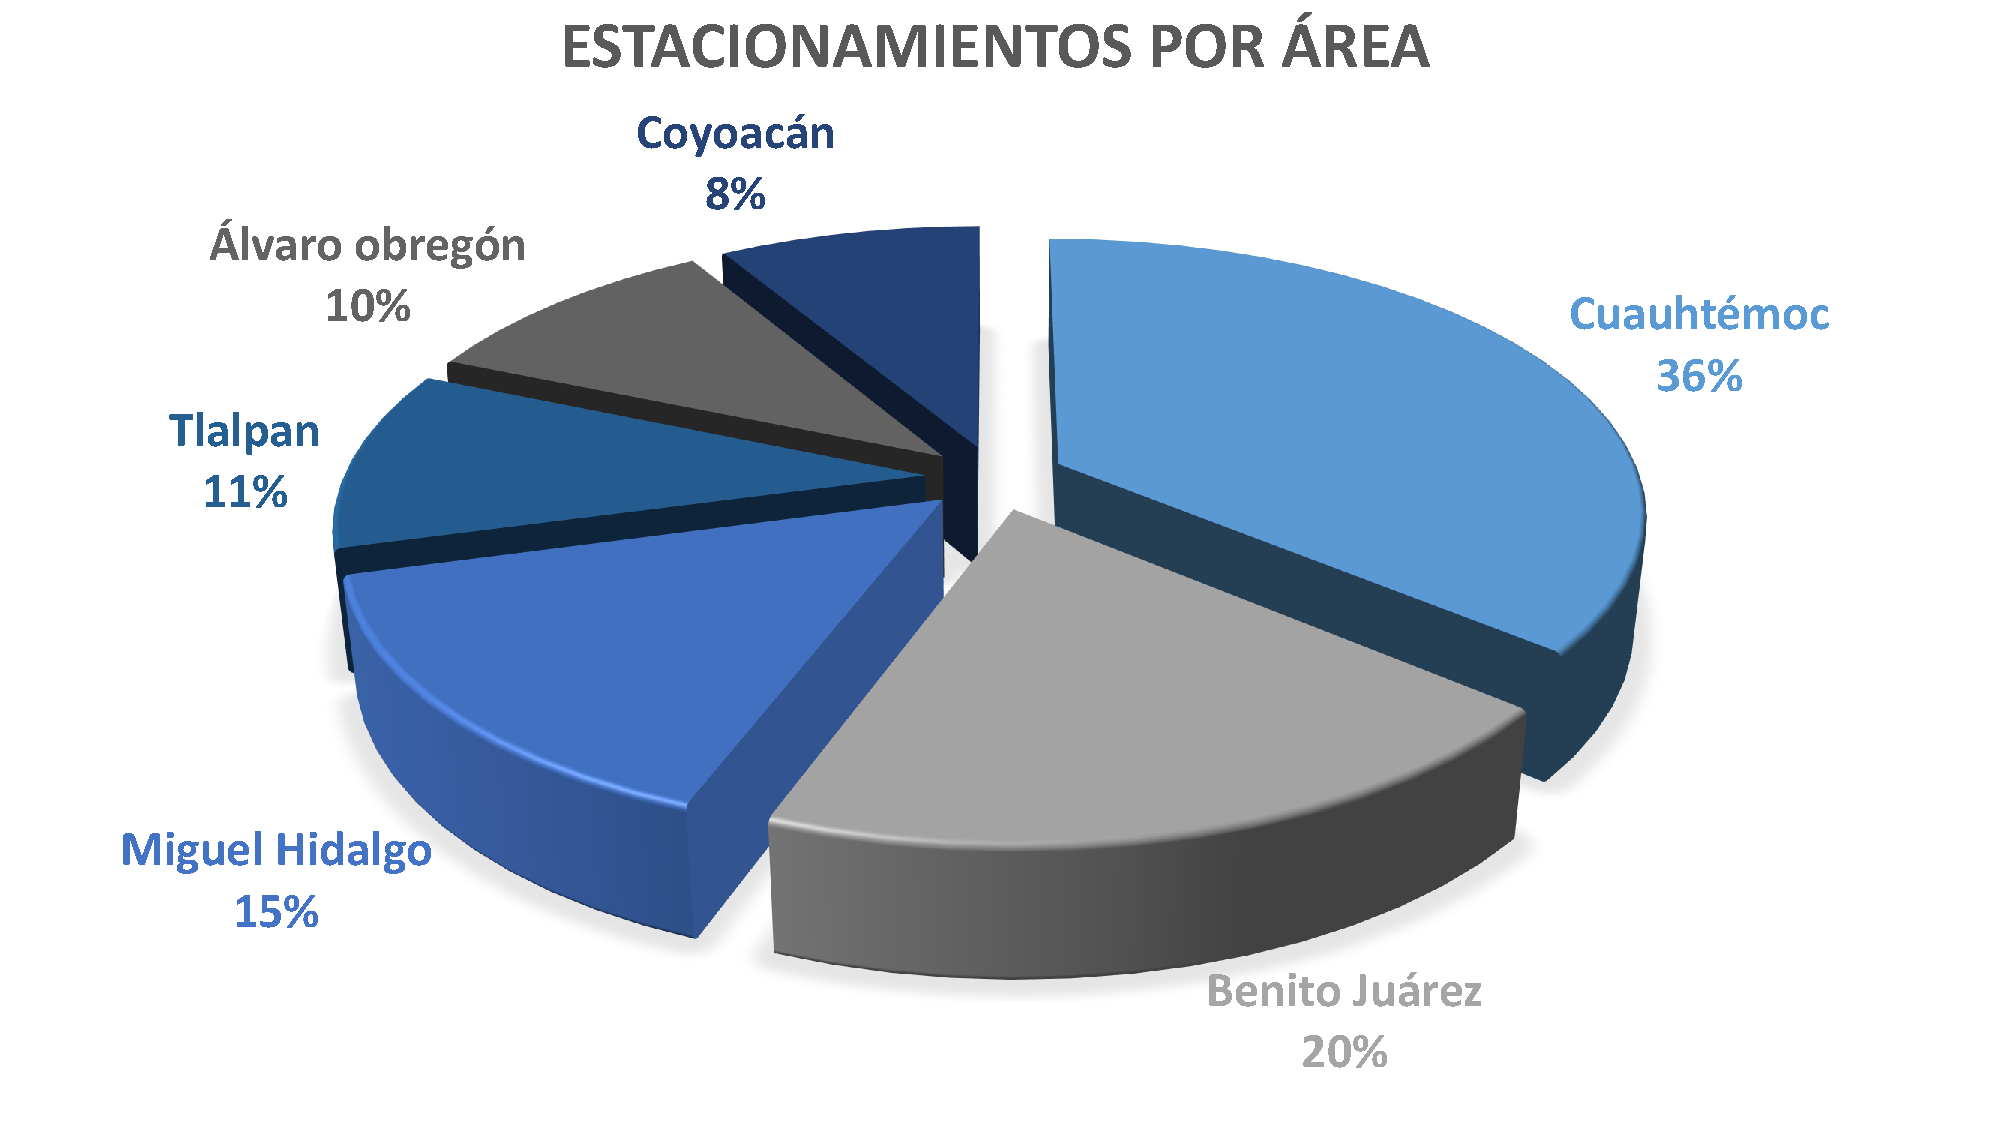
\includegraphics[scale=.3]{./analisisDeLaDemanda/source/estacionamientosPorArea}
	\caption{Estacionamientos por �rea en el DF}
	\label{fig:graficaEstacionamientosPorArea}
\end{figure}

\newpage

Otra opci�n para estacionar en veh�culo es el parqu�metro, datos obtenidos a trav�s de ecoParq (ecoparq, 2014), hay 1,229 parqu�metros instalados, atendiendo a 19,890 cajones en la v�a publica distribuidos de la como se muestra en el Cuadro \ref{tab:Parquimetros}.\\

\begin{table}
	\centering
	\begin{tabular}{|l|c|c|}
		\hline COLONIA & PARQUIMETRO & CAJONES \\ 
		\hline Anzures & 113 & 1695 \\ 
		\hline Lomas-Virreyes & 162 & 3250 \\ 
		\hline Nochebuena & 32 & 500 \\ 
		\hline Polanco & 416 & 6240 \\ 
		\hline Roma/Condesa & 353 & 5535 \\ 
		\hline Florencia & 85 & 1470 \\ 
		\hline Ciudad de los deportes & 40 & 760 \\ 
		\hline Cr�dito - Constructor & 28 & 440 \\ 
		\hline
	\end{tabular}
	\label{tab:Parquimetros}
	\caption{Parquimetros y cajones por Colonia.}
\end{table}

\newpage

Tomando como ejemplo la delegaci�n Cuauht�moc s�lo el 10.8\% de los autom�viles utilizan los aparcamientos p�blicos, mientras que 55.4\% aloja su veh�culo en estacionamientos privados, otro 28.5\% se estaciona en la v�a p�blica y s�lo 2.4\% de la poblaci�n lo hace en garaje propio (autobild, 2014).


\begin{figure}[h]
	\centering
	\includegraphics[scale=.3]{./analisisDeLaDemanda/source/TiposDeAlojamiento}
	\caption{Tipos de alojamiento, Delegacion Cuauht�moc}
	\label{fig:tiposDeAlojamiento}
\end{figure}


\subsection{Consumidores indirectos (usuarios finales)}
Seg�n datos del INEGI la flota  vehicular  registrada  en  el M�xico Distrito Federal se estima en 36.7 millones de veh�culos. (INEGI, 2013). 

\begin{figure}[h]
	\centering
	\includegraphics[scale=.4]{./analisisDeLaDemanda/source/VehiculosPorAno}
	\caption{Problemas cotidianos por falta de disponibilidad en estacionamietos}
	\label{fig:vehiculosPorAno}
\end{figure}

El tipo de demanda que se detecta es insatisfecha, ya que la gran mayor�a  de los estacionamientos (peque�os y medianos) opera solo con un dispositivo ?checador? que utilizan para contar el tiempo dentro del estacionamiento, y un registro  donde llevan el control de pensionados, y el total de las entradas diarias. 
Nosotros no centraremos en los estacionamientos peque�os y medianos ya que ellos representan un gran segmento del mercado y resulta muy favorable para el ellos el uso de SAE (GANAR-GANAR).

Existen otro tipo de estacionamientos, estos los podemos encontrar en centros comerciales, plazas, s�per mercados, cines, teatros, zonas, hospitales, etc. Estos estacionamientos los definimos con ?estacionamientos grandes?. Estos tienen la caracter�stica de tener mayores ingresos y por ende poseen una mejor infraestructura. Usualmente son administrador por un tercero y tiene sistema que automatiza las tareas operativas.  La desventaja principal de este tipo de estacionamientos es que el due�o del estacionamiento pierde el control del mismo y sus ingresos son   reducidos en gran medida, hasta de un 50\% de total, siempre y cuando el tercero haya recuperada la inversi�n inicial echa.  
Este tipo de estacionamientos no es nuestro principal cliente, pues ya posee un grado de automatizaci�n mayor; sin embargo SAE API brinda un conjunto de m�todos que pueden utilizar los sistemas externos para hacer uso de la plataforma que brinda SAE y con ellos aprovechar las ventajas que este brinda.

